\documentclass[a4paper,12pt]{report}
\usepackage[utf8]{inputenc}
\usepackage[T1]{fontenc}
\usepackage[french]{babel}
\usepackage{graphicx} 
\usepackage{hyperref} 
\hypersetup{
    colorlinks=true,    % Active la coloration du texte au lieu des cadres
    linkcolor=black,    % Couleur des liens internes (sections, sommaire)
    citecolor=black,    % Couleur des citations bibliographiques
    filecolor=black,    
    urlcolor=blue       % Couleur des liens vers le web (souvent gardée en bleu)
}
\usepackage{amsmath, amssymb} 
\usepackage{geometry}
\usepackage{float}
\usepackage{lmodern}
% Configuration des marges (un peu plus larges pour la reliure si impression)
\geometry{hmargin=2.5cm,vmargin=2.5cm}

\begin{document}

% --- DÉBUT DE LA PAGE DE GARDE PERSONNALISÉE ---
\begin{titlepage}
    % On passe en police Sans-Serif pour la couverture (plus moderne)
    \sffamily 
    \centering % Tout centrer par défaut

    % --- En-tête avec les logos ---
    % Utilisation de minipages pour aligner les logos gauche/droite
    \begin{minipage}{0.45\textwidth}
        \begin{flushleft}
            % Remplace par le nom exact de ton fichier image du badge "Licence IV"
            \includegraphics[height=2cm]{Université_Paris_8_Logo_2024.svg.png} 
        \end{flushleft}
    \end{minipage}
    \hfill
    \begin{minipage}{0.45\textwidth}
        \begin{flushright}
            % Remplace par le nom exact de ton fichier image "Paris 8"
            
\includegraphics[height=2cm]{logo.png} 
        \end{flushright}
    \end{minipage}

    \vspace{1.5cm}

    % --- Infos Université ---
    {\Large Université Paris 8}\\[0.2cm]
    {\large Licence Informatique \& Vidéoludisme}

    \vspace{2.5cm}

    % --- Titre du projet (Design moderne avec lignes horizontales) ---
    \rule{\linewidth}{0.5mm} \\[0.4cm] % Trait horizontal
    { \huge \bfseries Exploration du Langage et du Cerveau via l'Intelligence Artificielle \\[0.4cm] }
    \rule{\linewidth}{0.5mm} \\[1cm]

    % --- Type de document ---
    {\LARGE \textbf{Rapport de Projet Tutoré}}

    \vspace{3cm}

    % --- Étudiants et Tuteur ---
    % On sépare en deux colonnes
    \begin{minipage}{0.4\textwidth}
        \begin{flushleft} \large
            \emph{Réalisé par :}\\
            Nicolas \textsc{ROY}\\
            Theo \textsc{MASSENYA}
        \end{flushleft}
    \end{minipage}
    \hfill
    \begin{minipage}{0.4\textwidth}
        \begin{flushright} \large
            \emph{Tuteur :}\\
            Mme Revekka \textsc{KYRIAKOGLOU}
        \end{flushright}
    \end{minipage}

    \vfill % Pousse la date tout en bas de la page

    % --- Bas de page ---
    {\large Année universitaire 2025-2026}

\end{titlepage}
% --- FIN DE LA PAGE DE GARDE ---

% Remise de la police normale pour le reste du rapport
\normalfont 

% Table des matières
\tableofcontents

% --- AJOUT DE LA LISTE DES FIGURES ---
% C'est cette commande qui génère la liste automatiquement
\listoffigures 
% Ajoute la liste des figures à la table des matières (optionnel mais propre)
\addcontentsline{toc}{chapter}{Liste des figures} 

\newpage

% Inclusion des chapitres
\chapter*{Résumé}
\addcontentsline{toc}{chapter}{Résumé}

Ce projet tuteuré a pour objectif d'analyser le parallèle entre le traitement du langage par les modèles neuronaux de type Transformer et les mécanismes cognitifs du cerveau humain. Nous utilisons l'analyse de la dimensionnalité intrinsèque (ID) pour vérifier si l'IA effectue, comme le cerveau, une compression de l'information sémantique au cours de la lecture.

Pour répondre à cette problématique, nous formulons l'hypothèse que les phrases cohérentes créent une dynamique de «~ramping~» et un profil de compression spécifique (profil «~Hunchback~») qui seront absents ou modifiés lors du traitement de phrases «~Jabberwocky~» (syntaxiquement correctes mais dénuées de sens). Nous avons défini un protocole expérimental implémentant l'algorithme TwoNN sur le modèle GPT-2 pour mesurer ces variations géométriques couche par couche.

Dans le premier chapitre, nous explorons l'état de l'art en mettant en relation l'architecture des Transformers, le modèle neurolinguistique MUC et les propriétés mathématiques de l'ID. Puis, dans le chapitre suivant, nous détaillons notre méthodologie pour la phase d'expérimentation, en justifiant le choix de nos outils et la procédure de génération de nos stimuli linguistiques. Enfin, nous présentons dans le troisième chapitre notre feuille de route pour la mise en œuvre technique et l'analyse des résultats prévue au second semestre.
\chapter*{Introduction}
\addcontentsline{toc}{chapter}{Introduction} % Ajoute l'intro à la table des matières

Depuis l'introduction de l'architecture Transformer \cite{vaswani2017attention}, nous avons assisté à l'arrivée de modèles de langage de plus en plus performants. Initialement limités (comme GPT-2 ou BERT), ces modèles démontrent aujourd'hui des capacités linguistiques comparables, voire supérieures, à celles des humains sur certaines tâches spécifiques. Cependant, malgré ces performances, ces réseaux de neurones demeurent souvent des « boîtes noires » dont les mécanismes internes d'émergence du sens restent méconnus.

Dans le cadre de ce projet tuteuré, nous nous intéressons à la comparaison entre le fonctionnement de ces modèles artificiels et les mécanismes neurobiologiques du cerveau humain. Notre problématique centrale consiste à déterminer si l'Intelligence Artificielle traite la sémantique de manière analogue au cerveau, particulièrement en ce qui concerne l'unification des mots pour former une phrase cohérente. Pour ce faire, nous nous appuyons sur le modèle neurolinguistique MUC (\textit{Memory, Unification, Control}) \cite{hagoort2013memory} ainsi que sur une métrique issue de la géométrie de l'information : la dimensionnalité intrinsèque (ID) \cite{facco2017estimating, ansuini2019intrinsic}.

Pour mener à bien cette étude, nous avons choisi d'implémenter un environnement expérimental en Python, s'appuyant sur la librairie PyTorch. Nous utilisons le modèle GPT-2 pour son architecture causale (\textit{decoder-only}), proche de la linéarité de la lecture humaine. Nous utiliserons l'algorithme TwoNN \cite{facco2017estimating} pour estimer la complexité des représentations vectorielles (\textit{embeddings}) générées par le modèle. Afin d'isoler le traitement sémantique, nous avons élaboré un protocole comparant le traitement de phrases naturelles à celui de phrases de type « Jabberwocky » (syntaxiquement correctes mais dénuées de sens).

Ce rapport constitue la première partie de notre projet, focalisée sur l'étude théorique et la planification. Dans le premier chapitre, nous dressons un état de l'art reliant l'architecture des Transformers aux théories neurolinguistiques via le concept de dimensionnalité intrinsèque \cite{recanatesi2021predictive}. Dans le chapitre suivant, nous détaillons notre méthodologie et justifions nos choix d'implémentation. Enfin, nous présentons dans le troisième chapitre la feuille de route (\textit{roadmap}) détaillée de la phase d'expérimentation qui se déroulera au second semestre.
\chapter{État de l'art}
\label{chap:etat_art}

% --- CHAPEAU DU CHAPITRE (OBLIGATOIRE) ---
Dans ce chapitre, nous commençons par explorer l’architecture d’apprentissage profond des Transformers, sur laquelle repose la grande majorité des modèles actuels. Nous nous focaliserons particulièrement sur la manière dont ils représentent les mots via des représentations vectorielles appelées \textit{embeddings}. Puis, nous analyserons les mécanismes de traitement du langage dans le cerveau humain à travers le modèle récent du MUC. Nous verrons, enfin, comment il est possible d'établir un lien entre les dynamiques neuronales artificielles et biologiques grâce à la dimensionnalité intrinsèque (ID).

% --- SECTION 1.1 ---
\section{Les Modèles de Langage Neuronaux (NLMs)}
Cette section traite les concepts clés des Modèles de Langage Neuronaux (NLMs) nécessaires à la compréhension de ce projet. Elle décrit l’évolution technique apportée par les Transformers, la nature contextuelle des représentations vectorielles, et la manière dont l'apprentissage prédictif permet de "cristalliser" la structure sémantique du monde au sein d'une architecture neuronale.

\subsection{L'Architecture Transformer}
Introduite en 2017, l’architecture Transformer est aujourd’hui à la base de tous les principaux modèles de langage. Ce succès peut être attribué au mécanisme de \textit{Self-Attention}, qui permet au modèle de pondérer l'importance de chaque mot (ou token) de la séquence par rapport aux autres, quelle que soit leur distance \cite{vaswani2017attention}.

Cette approche est en rupture avec les modèles précédents (RNN/LSTM), basés sur des réseaux récurrents ou convolutifs qui traitaient les données de manière séquentielle. Dû à l’absence de ce traitement séquentiel dans les Transformers, il est nécessaire d’injecter des informations sur la position des tokens. Cela est réalisé via des \textit{positional encodings} ajoutés aux embeddings d’entrée \cite{vaswani2017attention}. C’est aussi cette absence de traitement séquentiel qui permet une parallélisation massive lors de l’entraînement, réduisant drastiquement les temps de calcul par rapport aux méthodes précédentes.

\subsection{Les Représentations Vectorielles (Embeddings)}
Les représentations vectorielles, ou \textit{embeddings}, sont le pivot entre le langage naturel et le traitement neuronal. Chaque token est projeté dans un espace continu de dimension $D_{model}$ (typiquement 512 dans le modèle original). Contrairement aux modèles statiques, les Transformers créent des représentations contextuelles où le vecteur évolue en fonction de l'environnement sémantique du mot.

Bien que ces vecteurs évoluent dans un espace de haute dimension, ils s'organisent sur des structures de dimensionnalité intrinsèque (ID) beaucoup plus faibles. Selon Recanatesi et al. (2021) \cite{recanatesi2021predictive}, l'apprentissage prédictif agit comme un mécanisme d'extraction de variables latentes, compressant les données sur des variétés de basse dimension qui encodent la structure sémantique du monde.

C'est la mesure de cette dimensionnalité "réelle" au sein des couches du modèle qui nous permettra, dans ce projet, de quantifier la complexité du traitement linguistique effectué par l'IA.

\subsection{L'Apprentissage Prédictif (Predictive Learning)}
La plupart des modèles de langage reposent sur l’apprentissage prédictif. Avec ce mécanisme, un réseau de neurones apprend à minimiser les erreurs entre sa sortie à un moment donné et un flux d'observations futures \cite{recanatesi2021predictive}. Pour un modèle de langage, cela se traduit par la prédiction du prochain token d’une séquence.

Pour réussir à anticiper le prochain token avec précision, le modèle doit extraire les structures logiques sous-jacentes au signal d’entrée (grammaire, sens des mots, contexte). Comme le soulignent Recanatesi et al. (2021) : \og \textit{Learning to predict observations about the world is a means for generating representations with easily accessed low-dimensional latent structure} \fg{}.

Cela crée un goulot d’étranglement (\textit{bottleneck}) : le réseau doit compresser des données d’entrée complexes en une représentation compacte qui ne contient que les informations nécessaires pour la prédiction future. Cette compression n’est pas qu’une réduction statistique, mais une réorganisation géométrique de l’information. En réduisant l'erreur de prédiction, le modèle projette des données sensorielles brutes vers des variétés (\textit{manifolds}) dont la courbure et la dimensionnalité reflètent la structure sémantique du monde \cite{recanatesi2021predictive}.

Néanmoins, l’étude de Desbordes et al. (2023) précise que lors du traitement d’une phrase, l’ID ne reste pas statique mais évolue mot après mot. Ils observent que les phrases porteuses de sens ont une ID plus élevée que les séquences dénuées de sens (type "Jabberwocky"). Cette perspective permet de considérer les modèles de langage comme des systèmes capables de "cristalliser" la structure du langage dans leur géométrie interne et non plus comme de simples prédicteurs statistiques.

% --- SECTION 1.2 ---
\section{La Dimensionnalité Intrinsèque (ID)}
Cette section présente la dimensionnalité intrinsèque (ID) appliqué aux architectures neuronales. Elle présente la méthode d'estimation TwoNN, l'évolution de l'ID à travers les couches du modèle (phénomène de "Hunchback"), et le rôle de l'apprentissage prédictif dans la création de variétés géométriques compactes et structurées. 

\subsection{Définition et Hypothèse de la Variété (Manifold Hypothesis)}
Pour comprendre comment les modèles structurent l'information, nous nous intéressons à la dimensionnalité intrinsèque (ID). Ce concept repose sur l'hypothèse de la variété (\textit{Manifold Hypothesis}) : bien que les données réelles soient encodées dans des espaces de haute dimension, elles sont en réalité contenues dans des variétés latentes de faibles dimensions \cite{facco2017estimating}.

L’ID correspond au nombre minimal de paramètres nécessaires pour décrire approximativement un ensemble de données. Pour l'estimer sans biais, Facco et al. (2017) ont proposé la méthode \textit{Two Nearest Neighbors} (TwoNN). Cette méthode, fonctionnant en mesurant le ratio des distances entre chaque point et ses deux voisins les plus proches, est aujourd’hui la référence du domaine.

\subsection{Dynamique de l'ID dans les Réseaux Profonds (Le profil "Hunchback")}
L’étude de Ansuini et al. (2019) \cite{ansuini2019intrinsic} a analysé l’évolution de l’ID à travers les couches des réseaux profonds (comme les CNNs). Ils ont mis en évidence que l’ID ne décroît pas de manière linéaire depuis l'entrée jusqu'à la sortie du modèle, mais observent plutôt un schéma \og bossu \fg{} (\textit{Hunchback}) récurrent. Ce schéma se décompose en deux phases distinctes :

\begin{itemize}
    \item \textbf{La phase d’expansion :} Dans les premières couches, l’ID augmente. Le réseau "déplie" les données pour les séparer et les analyser.
    \item \textbf{La phase de compression :} Une fois les données séparées, l’ID diminue progressivement dans les couches finales. Le réseau ne garde que l’information importante pour la tâche finale en éliminant le "bruit".
\end{itemize}
Ce phénomène est illustré par la Figure \ref{fig:hunchback}, où l'on observe clairement le pic de dimensionnalité dans les premières couches avant une chute progressive.

\begin{figure}[htbp]
    \centering
    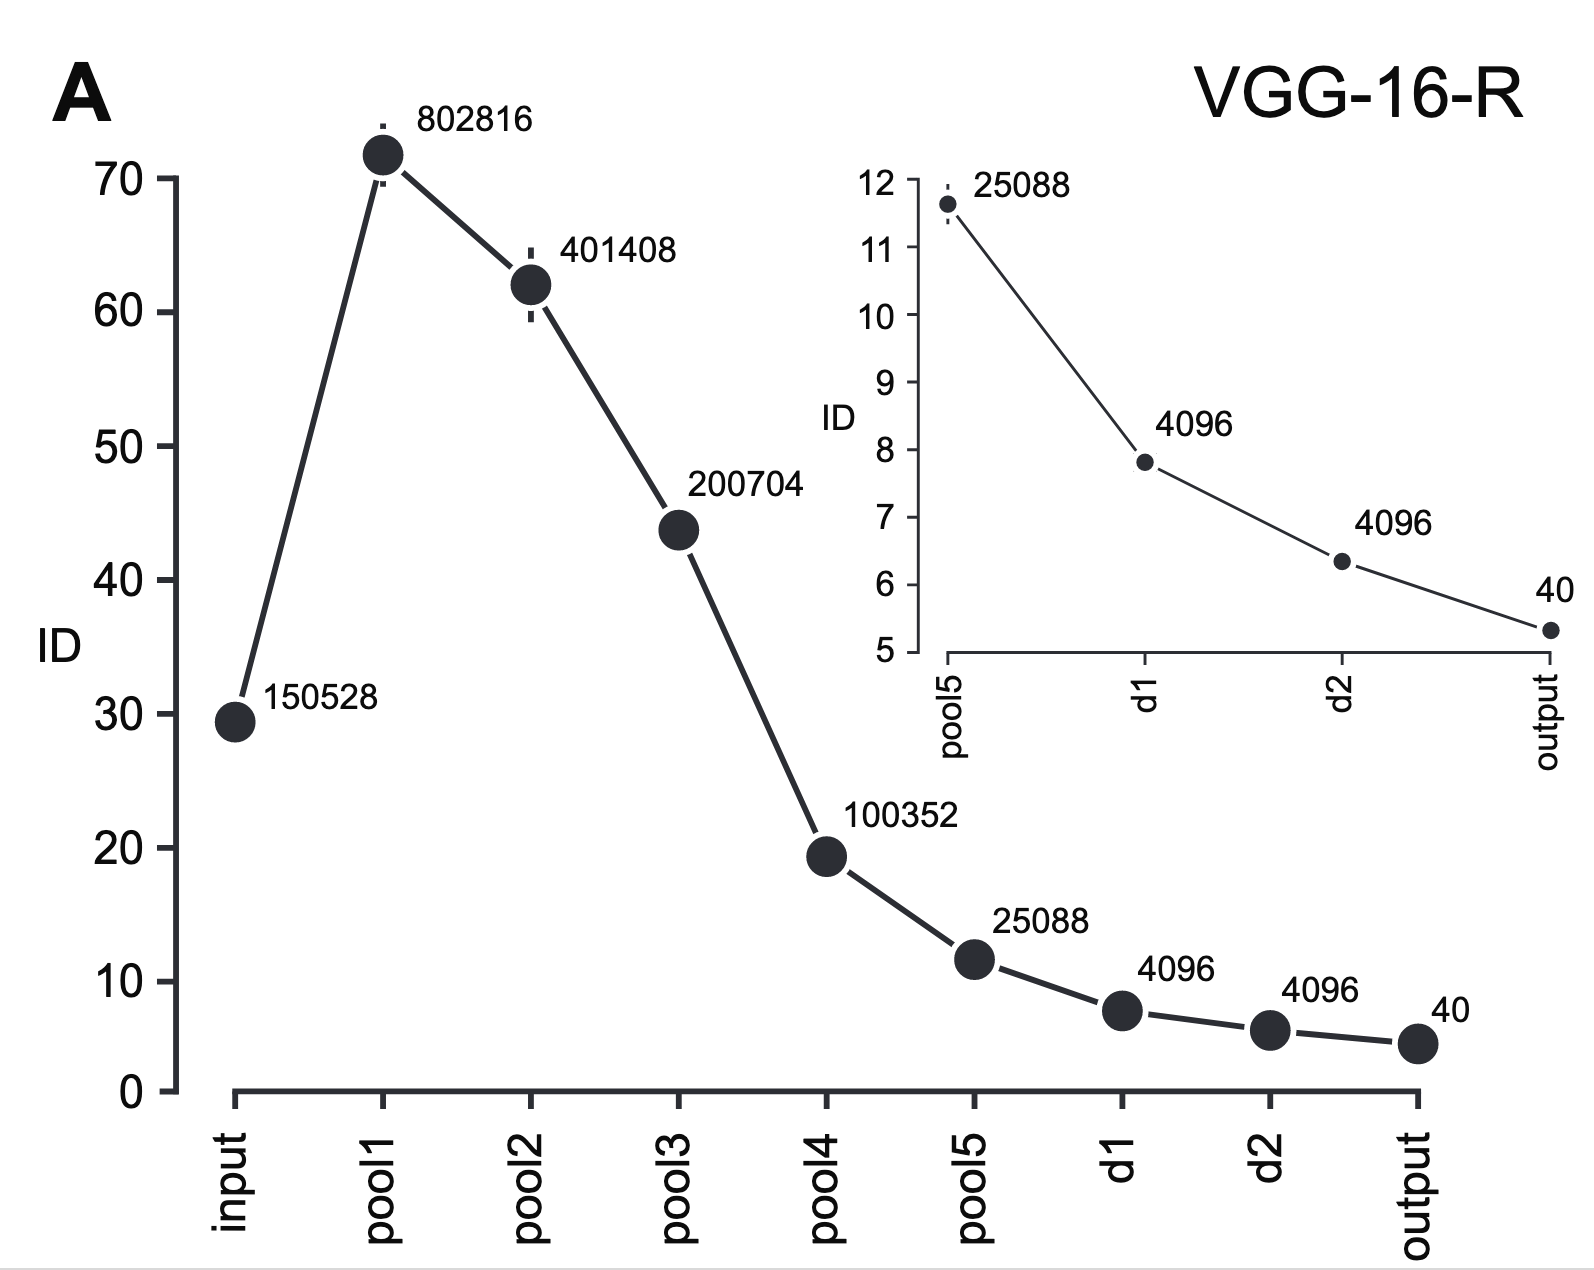
\includegraphics[width=0.5\linewidth]{profil Hunchback.png}
    \caption{Évolution de la Dimensionnalité Intrinsèque (ID) à travers les couches d'un réseau profond (VGG-16), illustrant le profil caractéristique « Hunchback » : une expansion suivie d'une compression. \textit{Source : Ansuini et al. [1]}}
    \label{fig:hunchback}
\end{figure}

Cela suggère que la performance d’un modèle provient de sa capacité à explorer la complexité d’un signal avant de le réduire en concepts abstraits de basse dimension.



\subsection{Mécanismes Prédictifs et ID}
Au-delà de l'observation, Recanatesi et al. (2021) lient l'émergence de ces structures de basse dimension au paradigme de l'apprentissage prédictif. Un point crucial soulevé par cette étude est la distinction entre deux types de mesures lors de l'apprentissage :

\begin{itemize}
    \item \textbf{La Dimensionnalité Linéaire (PR) :} Elle a tendance à augmenter ou rester élevée. Le réseau utilise un maximum d'espace pour "étaler" les représentations et les rendre facilement lisibles (linéairement séparables).
    \item \textbf{La Dimensionnalité Intrinsèque (ID non-linéaire) :} À l'inverse, celle-ci diminue drastiquement. C'est la preuve que les données, bien qu'étalées dans un grand espace, se concentrent sur une variété compacte.
\end{itemize}

Un gain élevé (rapport entre dimension linéaire et ID) signale que le modèle a construit une représentation robuste. Cela confirme que l'apprentissage prédictif force l'émergence de représentations structurées logiques, contrairement à d'autres méthodes comme l'auto-encodage simple.

% --- SECTION 1.3 ---
\section{Principes Neurolinguistiques et Parallèles IA}

Après avoir étudié les Transformers et l'ID, nous allons nous intéresser aux bases neurobiologiques du langage qui permettent au cerveau de construire le sens. Le traitement du langage par le cerveau est une fonction cognitive complexe impliquant de faire fonctionner ensemble la mémoire, l’attention et des processus combinatoires.

\subsection{Le Modèle MUC : Mémoire, Unification, Contrôle}
Le modèle dominant actuel est le \textit{Memory, Unification, and Control} (MUC) proposé par Peter Hagoort \cite{hagoort2013memory}. Il vient remplacer le modèle de Wernicke-Lichtheim-Geschwind, qui se focalise sur le mot unique. Le MUC structure le traitement linguistique en trois composantes distinctes mais interactives :

\begin{itemize}
    \item \textbf{Mémoire (Memory) :} C’est la composante qui va servir au stockage et à la récupération des connaissances linguistiques acquises (formes phonologiques, morphologiques, cadres syntaxiques). Elle est principalement localisée dans le cortex temporal gauche en jaune sur la Figure \ref{fig:muc_brain}.
    \item \textbf{Unification :} L'unification est l'assemblage dynamique des briques lexicales récupérées en mémoire pour former des structures cohérentes. Ce processus se déroule principalement dans le gyrus frontal inférieur gauche (aire de Broca) représentée en bleu sur la Figure \ref{fig:muc_brain}. C'est ici que la syntaxe et la sémantique fusionnent pour construire une représentation unifiée. 
    \item \textbf{Contrôle (Control) :} Cette composante gère l'attention, le tour de parole et la sélection de la langue pertinente, impliquant le cortex préfrontal dorsolatéral en rose sur la Figure \ref{fig:muc_brain}.
\end{itemize}

\begin{figure}[H] % On remplace [htbp] par [H]
    \centering
    % Remplacez 'nom_de_l_image_cerveau' par le vrai nom du fichier
    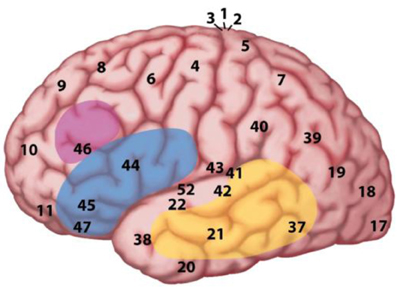
\includegraphics[width=0.5\textwidth]{The-MUC-model-of-language-The-figure-displays-a-lateral-view-of-the-left-hemisphere-The.png}
    
    % La légende simplifiée pour aller à l'essentiel
    \caption{Localisation anatomique des composantes du modèle MUC dans l'hémisphère gauche. En jaune : la Mémoire (cortex temporal). En bleu : l'Unification (aire de Broca). En rose : le Contrôle (cortex préfrontal). \textit{Source : Hagoort [5]}}
    
    \label{fig:muc_brain}
\end{figure}

L’unification implique que le cerveau maintient une représentation active qui croît en complexité à mesure que de nouveaux mots sont intégrés. Cette charge cognitive croissante devrait, selon notre hypothèse, se refléter dans la dimensionnalité de l'activité neuronale (et artificielle).

\subsection{Signatures Dynamiques : Le "Ramping" et l'Intégration}
Des études récentes (Fedorenko et al., 2016 \cite{fedorenko2016broad} ; Desbordes et al., 2023 \cite{desbordes2023}) ont identifié des marqueurs temporels de cette unification : l'activité de \textit{ramping}, une augmentation lente et continue de la puissance neuronale au cours de la phrase.

Ce signal ne répond pas simplement à chaque mot individuellement (activité phasique), mais semble accumuler l'information contextuelle. Les expériences utilisant des paradigmes "Jabberwocky" (phrases syntaxiquement correctes mais sans sens) révèlent que si la structure syntaxique seule crée une activité, les phrases sensées génèrent un \textit{ramping} beaucoup plus soutenu. Ce phénomène est également observé par Desbordes et al. (2023) dans les modèles artificiels.

% --- SECTION 1.4 ---
\section{Synthèse et Hypothèses de Travail}

En croisant ces trois domaines (Transformers, ID, Neurolinguistique), nous formulons les hypothèses qui guideront notre méthodologie pour la suite de ce projet :

\begin{enumerate}
    \item Les modèles de langage, comme le cerveau, présentent une activité de \textit{ramping} au cours de la lecture d'une phrase.
    \item La dimensionnalité intrinsèque des représentations augmentera plus fortement pour les phrases sémantiquement cohérentes que pour les phrases Jabberwocky, reflétant le coût computationnel de l'unification sémantique.
    \item Le profil de l'ID à travers les couches des Transformers montrera une expansion suivie d'une compression (profil \textit{Hunchback}), mais cette dynamique sera perturbée par les stimuli Jabberwocky, le modèle échouant à converger vers une représentation stable faute de sens.
\end{enumerate}

% --- CONCLUSION DU CHAPITRE (OBLIGATOIRE) ---
Dans ce chapitre, nous avons posé les bases théoriques liant l'architecture des Transformers aux théories neurolinguistiques via l'analyse de la dimensionnalité intrinsèque. Ces éléments constituent le fondement de notre approche expérimentale, dont nous détaillerons la méthodologie et l'implémentation dans le chapitre suivant.
\chapter{Méthodologie et Implémentation}
\label{chap:methode}

% --- CHAPEAU DU CHAPITRE ---
Dans ce chapitre, nous justifions nos choix d'implémentation afin de vérifier les trois hypothèses formulées précédemment. Ces choix résultent directement des constats de l'état de l'art. Nous détaillerons d'abord l'architecture technique retenue, puis le protocole rigoureux de création des stimuli linguistiques, pour enfin exposer les étapes d'analyse nous permettant de mesurer la dimensionnalité intrinsèque.

% --- SECTION 2.1 ---
\section{Justification des Choix Techniques}

Afin de mesurer l'évolution de la dimensionnalité intrinsèque (ID) au sein d'une architecture neuronale, nous avons sélectionné un ensemble d'outils spécifiques.

\subsection{Modèle de Langage : GPT-2 Small}
Nous avons choisi GPT-2 (via la librairie \textit{HuggingFace}) en raison de son architecture \textit{Decoder-only} qui traite l'information de manière unidirectionnelle (de gauche à droite, avec un masque causal). Ce choix est crucial pour tester l'activité de \textit{ramping} (Hypothèse 1), car il simule la progression temporelle de la lecture humaine, contrairement aux modèles bidirectionnels comme BERT qui "voient" toute la phrase d'un coup.

\subsection{Algorithme d'Estimation de l'ID : TwoNN}
Conformément à l'état de l'art établi par Facco et al. (2017) \cite{facco2017estimating}, nous utiliserons l'algorithme \textit{Two-Nearest Neighbors} (TwoNN). 

Son principal avantage est sa robustesse face aux variations de densité des données. Comme nous travaillons sur des variétés (\textit{manifolds}) locales (mot par mot), TwoNN permet d'estimer l'ID sans être biaisé par la courbure globale de l'espace des embeddings.
Le principe est le suivant : pour chaque point $i$ (représentation d'un token), on calcule les distances vers ses deux plus proches voisins, $r_{i,1}$ et $r_{i,2}$.

\subsection{Langage et Frameworks}
L’implémentation est réalisée en \textbf{Python}. Nous utilisons :
\begin{itemize}
    \item \textbf{PyTorch} pour l’extraction des \textit{hidden states} (états cachés) à chaque couche du modèle.
    \item \textbf{NumPy} pour la manipulation des données multidimensionnelles, le calcul matriciel et la gestion des tenseurs.
    \item \textbf{scikit-dimension} qui fournit une implémentation optimisée de l'algorithme TwoNN.
\end{itemize}

\subsection{Extension vers Llama 3.1 (8B)}
Nous intégrons également un modèle récent, Llama 3.1 (8 milliards de paramètres), pour généraliser nos observations. Cela nous permettra de prouver que les mécanismes de compression sémantique sont fondamentaux aux architectures Transformers modernes, et d'observer si la "vitesse" de compression diffère selon la profondeur du modèle.

\subsection{Limites de la modélisation du MUC}
Il est important de noter une limite théorique : l’architecture Transformer ne modélise pas la composante \og Contrôle \fg{} du modèle MUC. Dans le cerveau humain, le contrôle intervient pour résoudre les conflits sémantiques (comme face au Jabberwocky). Ici, GPT-2 et Llama 3 n’ont pas de supervision ; ils traiteront le Jabberwocky comme une séquence statistique improbable. Nous nous attendons donc à voir l’échec de l’Unification (un profil \textit{Hunchback} déformé) sans pouvoir observer l’activité compensatoire du Contrôle.

% --- SECTION 2.2 ---
\section{Protocole de Génération des Stimuli}

La validation de nos hypothèses repose sur la comparaison de deux types de signaux. L’objectif est d’isoler l’impact du sens (la sémantique) en maintenant la structure grammaticale constante.

\subsection{Le groupe "Sémantique"}
Nous avons constitué un corpus de \textbf{500 phrases} extraites du dataset \textit{Wikitext} (Wikipedia). Ce volume a été choisi pour deux raisons :
\begin{itemize}
    \item \textbf{Stabilité statistique :} L'estimateur TwoNN nécessite une densité de points suffisante pour éviter les biais. 500 phrases permettent d'obtenir une courbe d'évolution de l'ID représentative.
    \item \textbf{Diversité linguistique :} Ce nombre couvre une variété de structures syntaxiques (phrases simples, complexes, énumérations), évitant le biais d'un style d'écriture spécifique.
\end{itemize}

\subsection{Le groupe "Jabberwocky"}
Pour tester l'Hypothèse 3, nous avons généré une version "vide de sens" de chaque phrase du premier groupe. Ce procédé s'inspire des neurosciences cognitives pour tromper le modèle sans briser la structure de la langue.

Le processus de transformation suit trois règles strictes :
\begin{enumerate}
    \item \textbf{Préservation des mots-outils :} Nous conservons les déterminants, prépositions et conjonctions (ex: le, la, dans, mais) qui servent de squelette syntaxique.
    \item \textbf{Substitution lexicale :} Seuls les mots porteurs de sens (noms, verbes, adjectifs) sont remplacés.
    \item \textbf{Respect de la phonotactique :} Les pseudo-mots (ex: \textit{vlipure, carlouée}) sont créés pour respecter les règles de sonorité du français. Ils sont "lisibles" mais n'existent pas dans le dictionnaire du modèle.
\end{enumerate}

\textit{Exemple :} "La musique d'Elsa Barraine est rarement jouée" devient "La vlipure d'Elsa Barraine est jitrement carlouée".

\subsection{Synthèse des données}
Chaque phrase "Jabberwocky" possède exactement le même nombre de mots et la même structure grammaticale que sa phrase "Sémantique" correspondante. Cette approche par paires garantit que toute différence de dimensionnalité observée est uniquement due à l'absence de cohérence sémantique.

\subsection{Enjeux de la Tokenisation (BPE)}
Avant d'être traitées, les phrases sont converties en unités numériques par l'algorithme \textit{Byte Pair Encoding} (BPE). Ce processus est crucial et induit un biais technique pour le Jabberwocky :
\begin{itemize}
    \item \textbf{Fragmentation :} Les mots du groupe "Sémantique" existent dans le vocabulaire et forment souvent un seul token. Les pseudo-mots (ex: \textit{vlipure}) sont inconnus et sont fragmentés en sous-unités (ex: \textit{vli + pure}).
    \item \textbf{Conséquence :} Cette fragmentation augmente mécaniquement le nombre de pas de temps. Nous devrons analyser l'évolution de l'ID de manière relative à la progression dans la phrase, car le modèle fournit un effort supplémentaire de reconstruction pour lier ces fragments.
\end{itemize}

% --- SECTION 2.3 ---
\section{Étapes de l'analyse}

Pour chaque phrase testée, nous suivons un parcours précis d'observation :

\begin{itemize}
    \item \textbf{Récupération de l'activité interne :} Nous n'observons pas seulement la sortie, mais nous enregistrons l'activité des \textit{hidden states} à chaque couche intermédiaire. Cela nous donne une image précise de l'état du modèle, mot après mot.
    
    \item \textbf{Mesure de l'ID mot après mot :} Pour tester l'effet de \textit{ramping}, nous calculons la dimensionnalité au fur et à mesure que le modèle lit la phrase (1er mot, puis 1er+2ème, etc.). Cela permet de voir si l'information s'accumule ou stagne.
    
    \item \textbf{Comparaison des profils de couches :} Nous comparons l'évolution de la complexité entre l'entrée et la sortie. L'objectif est de vérifier si le modèle parvient à compresser les phrases sémantiques (profil d'expansion-compression).
\end{itemize}

À l'inverse, avec le Jabberwocky, nous nous attendons à ce que cette simplification échoue. Comme le mot "vlipure" ne correspond à rien de connu, le modèle ne peut pas le compresser vers un concept simple. Il reste "perdu" dans la complexité, ce qui devrait empêcher la chute de l'ID dans les dernières couches.

% --- CONCLUSION DU CHAPITRE (OBLIGATOIRE) ---
Dans ce chapitre, nous avons détaillé notre approche méthodologique, justifiant le choix des modèles (GPT-2, Llama) et de la métrique (TwoNN). Nous avons également défini un protocole strict de génération de stimuli (Sémantique vs Jabberwocky) pour isoler l'impact du sens sur la dimensionnalité. Ces outils et ces données sont maintenant prêts à être utilisés pour générer les résultats que nous analyserons dans le chapitre suivant.
\chapter{Planification et Roadmap}

% Chapeau du chapitre (Obligatoire selon le modèle du mémoire)
Dans ce chapitre, nous présentons l'organisation du projet au cours du second semestre. Notre travail va se diviser en quatre phases principales, allant de la mise en place technique jusqu'à la rédaction finale. Cette planification assure une progression logique, de la validation des outils à l'interprétation des données neurolinguistiques.

\section{Mise en place de l'environnement technique et Génération des Stimuli (Février)}

L'objectif de cette première phase est de disposer d'un pipeline fonctionnel pour la création du dataset et la validation des métriques avant de lancer les calculs lourds.

\subsection{Mise en place de l'environnement technique}
Nous procéderons d'abord à l'initialisation de l'espace de travail :
\begin{itemize}
    \item \textbf{Installation et configuration} des librairies essentielles : PyTorch (calcul tensoriel), Hugging Face Transformers (modèles de langage) et scikit-dimension (calcul de l'ID).
    \item \textbf{Test de chargement} des modèles (GPT-2 Small) pour s'assurer de leur bon fonctionnement en local.
\end{itemize}

\subsection{Écriture d'un générateur de Jabberwocky}
Cette étape est cruciale pour la validation de nos hypothèses sémantiques, Le fonctionnement attendu du générateur est détaillé dans la Figure \ref{fig:jabberwocky_process}, qui montre comment la structure syntaxique est préservée lors de la substitution lexicale.

\begin{itemize}
    \item \textbf{Développement du script} de transformation des phrases du groupe « Sémantique » vers le groupe « Jabberwocky ». Ce script appliquera les règles définies dans la méthodologie : préservation stricte des mots-outils et substitution lexicale respectant la phonotactique anglaise.
    \item \textbf{Vérification manuelle} d'un échantillon aléatoire pour garantir que la structure grammaticale est conservée malgré la perte de sens.
\end{itemize}

\begin{figure}[H] 
    \centering

    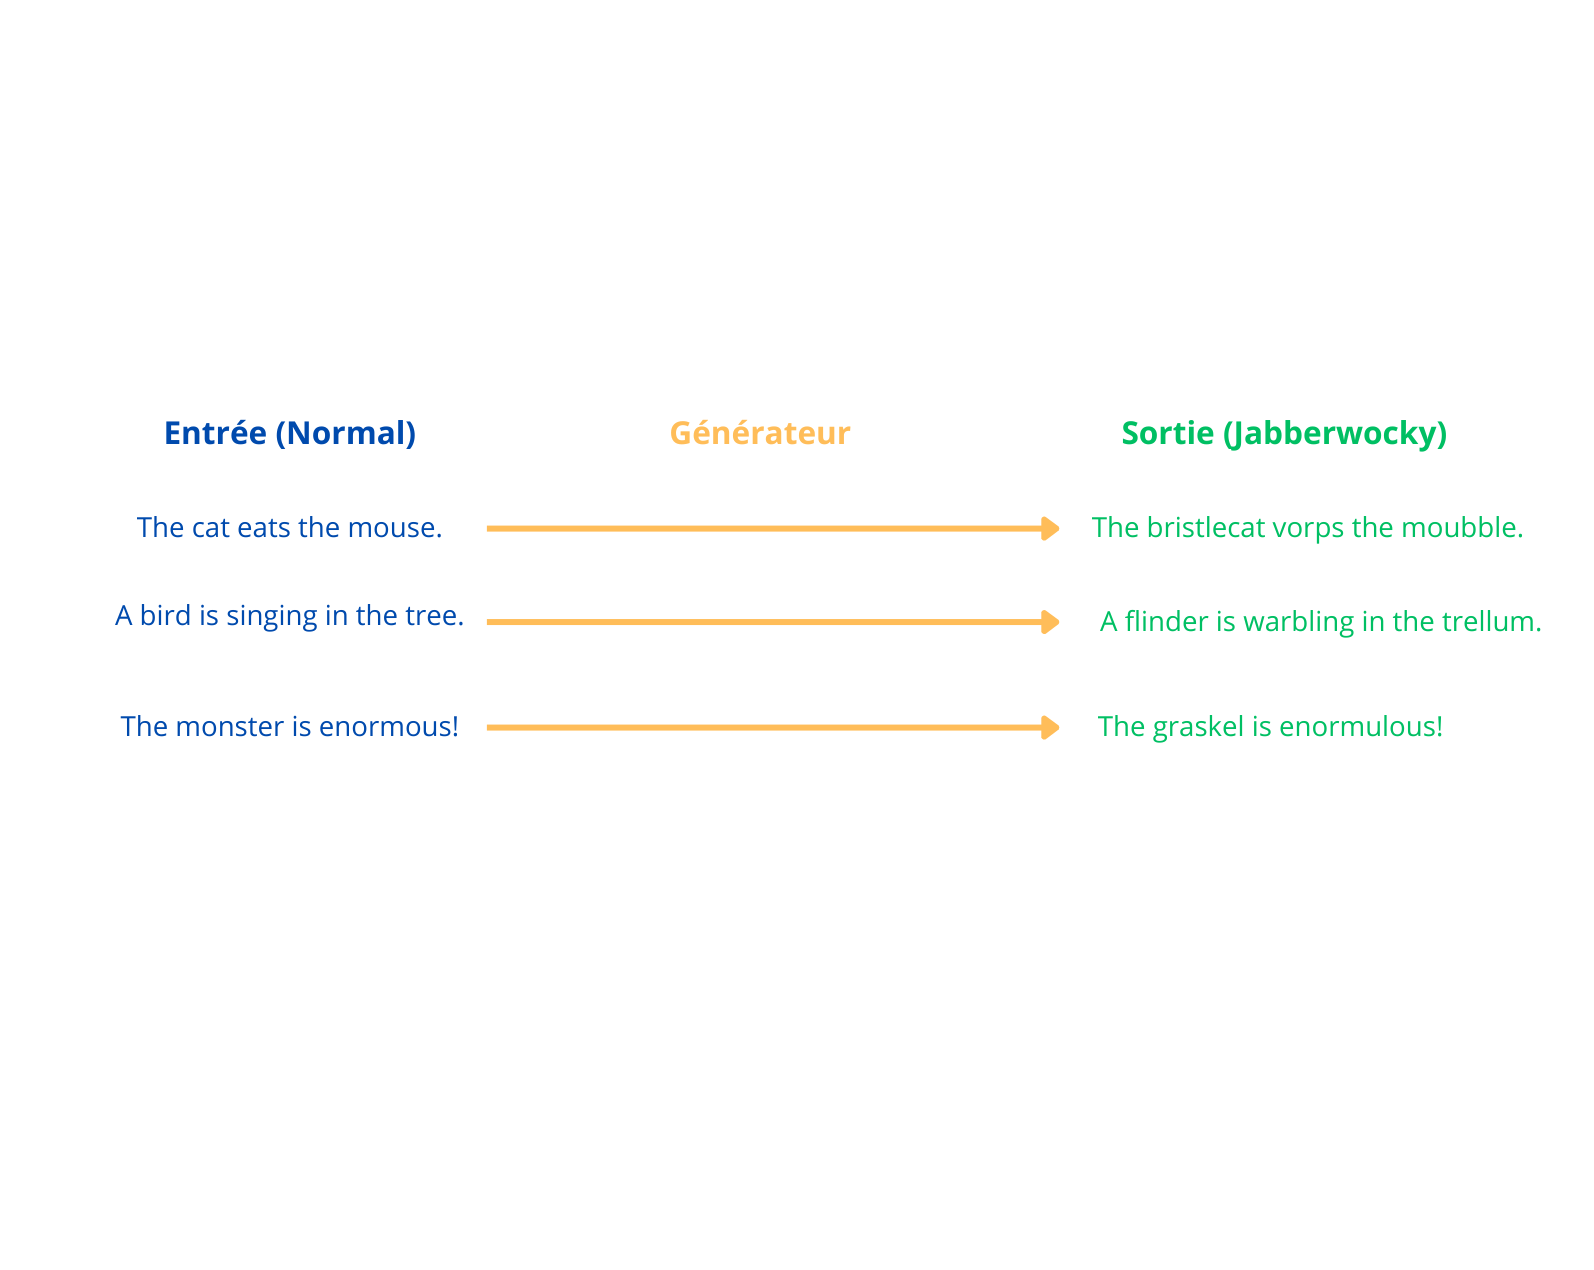
\includegraphics[width=0.9\textwidth]{Le_Jabberwocky_(en).png}
    
    \caption{Illustration du processus de génération des stimuli « Jabberwocky ». Le générateur conserve les mots-outils (en bleu) mais remplace les mots lexicaux par des pseudo-mots (en vert) respectant la phonotactique. \textit{Source : Production personnelle}}
    
    \label{fig:jabberwocky_process}
\end{figure}

\subsection{Validation et tests de TwoNN}
Avant d'analyser les embeddings, nous devons calibrer notre instrument de mesure :
\begin{itemize}
    \item \textbf{Tests de l'algorithme TwoNN} sur des variétés synthétiques dont la dimension est connue (ex: hypersphère). Cela nous permettra d'ajuster les hyperparamètres (nombre de voisins $k$) avant l'application sur les données réelles.
\end{itemize}

\section{Expérimentation Principale (Mars)}

L'objectif de cette phase est de tester les Hypothèses 1 (Ramping) et 2 (Impact Sémantique) définies dans le premier chapitre.

\subsection{Extraction et Tokenisation}
Le traitement des données suivra le protocole suivant :
\begin{itemize}
    \item \textbf{Passage des phrases} dans le tokenizer BPE (Byte Pair Encoding).
    \item \textbf{Normalisation temporelle} : mise en place d'une méthode pour pallier les disparités de longueur des séquences, dues à la fragmentation plus importante des pseudo-mots (Jabberwocky) par le tokenizer.
\end{itemize}

\subsection{Calcul de la Dimensionnalité Intrinsèque}
C'est le cœur de notre expérience technique :
\begin{itemize}
    \item \textbf{Enregistrement des états cachés} (hidden states) couche par couche, lors de l'exécution du modèle (forward pass).
    \item \textbf{Calcul de l'ID via TwoNN} mot après mot (approche incrémentale) pour visualiser la dynamique temporelle de l'intégration de l'information.
\end{itemize}

\subsection{Analyse des profils de « Ramping »}
Une fois les données brutes obtenues, nous passerons à l'analyse :
\begin{itemize}
    \item \textbf{Comparaison statistique} des pentes d'ID entre le groupe Sémantique et le groupe Jabberwocky.
    \item \textbf{Vérification de l'hypothèse} d'une accumulation d'informations (ramping) significativement plus soutenue pour les phrases porteuses de sens.
\end{itemize}

\section{Analyse Structurelle et Extension (Mars)}

Dans cette troisième phase, l'objectif est de tester l'Hypothèse 3 (Profil Hunchback) et de tenter une généralisation des résultats sur une architecture plus récente (Llama 3.1).

\subsection{Étude du profil Hunchback sur GPT-2}
Nous chercherons à valider la théorie de la compression de l'information :
\begin{itemize}
    \item \textbf{Agrégation des IDs moyens} par couche, de l'entrée (embedding layer) à la sortie (prediction head).
    \item \textbf{Identification des phases} d'expansion et de compression caractéristiques du profil Hunchback.
    \item \textbf{Observation des anomalies} : nous analyserons spécifiquement la déformation de ce profil (potentiel échec de compression) sur le dataset Jabberwocky.
\end{itemize}

\subsection{Réplication sur Llama 3.1}
Pour assurer la robustesse de nos conclusions :
\begin{itemize}
    \item \textbf{Adaptation du code} pour gérer l'inférence sur Llama 3.1 (modèle de 8 milliards de paramètres).
    \item \textbf{Comparaison inter-modèles} : nous comparerons les résultats avec GPT-2 pour déterminer si la « profondeur » du modèle ou sa taille influence la vitesse et l'efficacité de la compression sémantique.
\end{itemize}

\section{Interprétation et Rédaction (Avril)}

La phase finale consistera à synthétiser les résultats et à les confronter au modèle neurolinguistique MUC.

\subsection{Visualisation des données}
La production de supports graphiques sera prioritaire pour le rapport final :
\begin{itemize}
    \item \textbf{Création de graphes comparatifs} montrant les courbes d'évolution de l'ID au cours du temps (pour le ramping) et à travers les couches (pour le profil Hunchback).
\end{itemize}

\subsection{Analyse critique}
Enfin, nous rédigerons l'analyse finale :
\begin{itemize}
    \item \textbf{Discussion des résultats} au regard des hypothèses initiales.
    \item \textbf{Traitement des limites} : nous discuterons notamment de l'absence du mécanisme de « Contrôle » (au sens du modèle MUC) dans les modèles de langage actuels et son impact sur le traitement des phrases absurdes.
\end{itemize}
\chapter*{Conclusion} % L'étoile évite la numérotation mais l'affiche

Dans ce rapport, nous avons posé les fondements théoriques et méthodologiques nécessaires à notre étude comparant le traitement du langage par les modeles basé sur l'architecture des transformers aux cerveau humain. 



Dans un premier temps, notre état de l'art a mis en évidence les similitudes de l'architecture des Transformers avec le modèle neurolinguistique MUC (Mémoire, Unification, Contrôle). Nous avons montré que l'apprentissage prédictif force les modèles à compresser l'information sémantique sur des variétés de basse dimension, un mécanisme que nous supposons similaire a la composante d'unification du MUC.



Sur le plan méthodologique, nous avons justifié le choix de l'algorithme TwoNN afin de mesurer cette compression. Bien que cet algorithme puisse présenter des instabilités sur de très petits échantillons, sa robustesse face aux courbures locales en fait l'outil le plus adapté à notre étude couche par couche. 

Nous avons aussi détaillé notre protocole de génération de stimuli, comparant des phrases sémantiques à des séquences "Jabberwocky". Dans le but de pouvoir isoler l'impact du sens sur la géométrie des représentations.



 Nous avons établi une roadmap détaillée de la phase d'implémentation au cours du semestre prochain, de la validation technique des scripts en février jusqu'à l'analyse critique des résultats en avril.



Cette phase d'implémentation consistera à vérifier l'existence du phénomène de « ramping » et à observer la déformation du profil de Hunchback dans le traitement de phrase dénué de sens.

\addcontentsline{toc}{chapter}{Conclusion et Perspectives}

% Bibliographie
\bibliographystyle{alpha}
\bibliography{references}

\end{document}